\chapter{Diagrama de Nodos}
\section{Definición}
Un Diagrama de Nodos modela la arquitectura en tiempo de ejecución de un sistema. Esto muestra la configuración de los elementos de hardware (nodos) y muestra cómo los elementos y artefactos del software se trazan en esos nodos.

\subsection*{Nodo}
Un Nodo es un elemento de hardware o software. Esto se muestra con la forma de una caja en tres dimensiones, como a continuación.

\subsection*{Instancia de Nodo}
Una instancia de nodo se puede mostrar en un diagrama. Una instancia se puede distinguir desde un nodo por el hecho de que su nombre esta subrayado y tiene dos puntos antes del tipo de nodo base. Una instancia puede o no tener un nombre antes de los dos puntos. El siguiente diagrama muestra una instancia nombrada de una computadora.

\subsection*{Asociación}
En el contexto del diagrama de despliegue, una asociación representa una ruta de comunicación entre los nodos. El siguiente diagrama muestra un diagrama de despliegue para una red, mostrando los protocolos de red como estereotipos y también mostrando multiplicidades en los extremos de la asociación.

\subsection*{Nodo como contenedor}
Un nodo puede contener otros elementos, como componentes o artefactos. El siguiente diagrama muestra un diagrama de despliegue para una parte del sistema embebido y muestra un artefacto ejecutable como contenido por el nodo madre (motherboard).

\section{Implementación}
Para el caso concreto del proyecto en desarrollo, se plantea una estructura de cliente-servidor a nivel de bases de datos; la información estará almacenada en una base de datos puesta en un servidor mientras que por  parte del cliente, existirán 2 herramientas cliente: una de tipo \textbf{Administrativa} y otra dirigida a los \textbf{Clientes finales}. Dichas herramientas se conectarán de forma remota al servidor para la interacción de los usuarios con la información. En la siguiente imagen se expone la implementación mencionada:

\begin{figure}[h!]
	\centering
	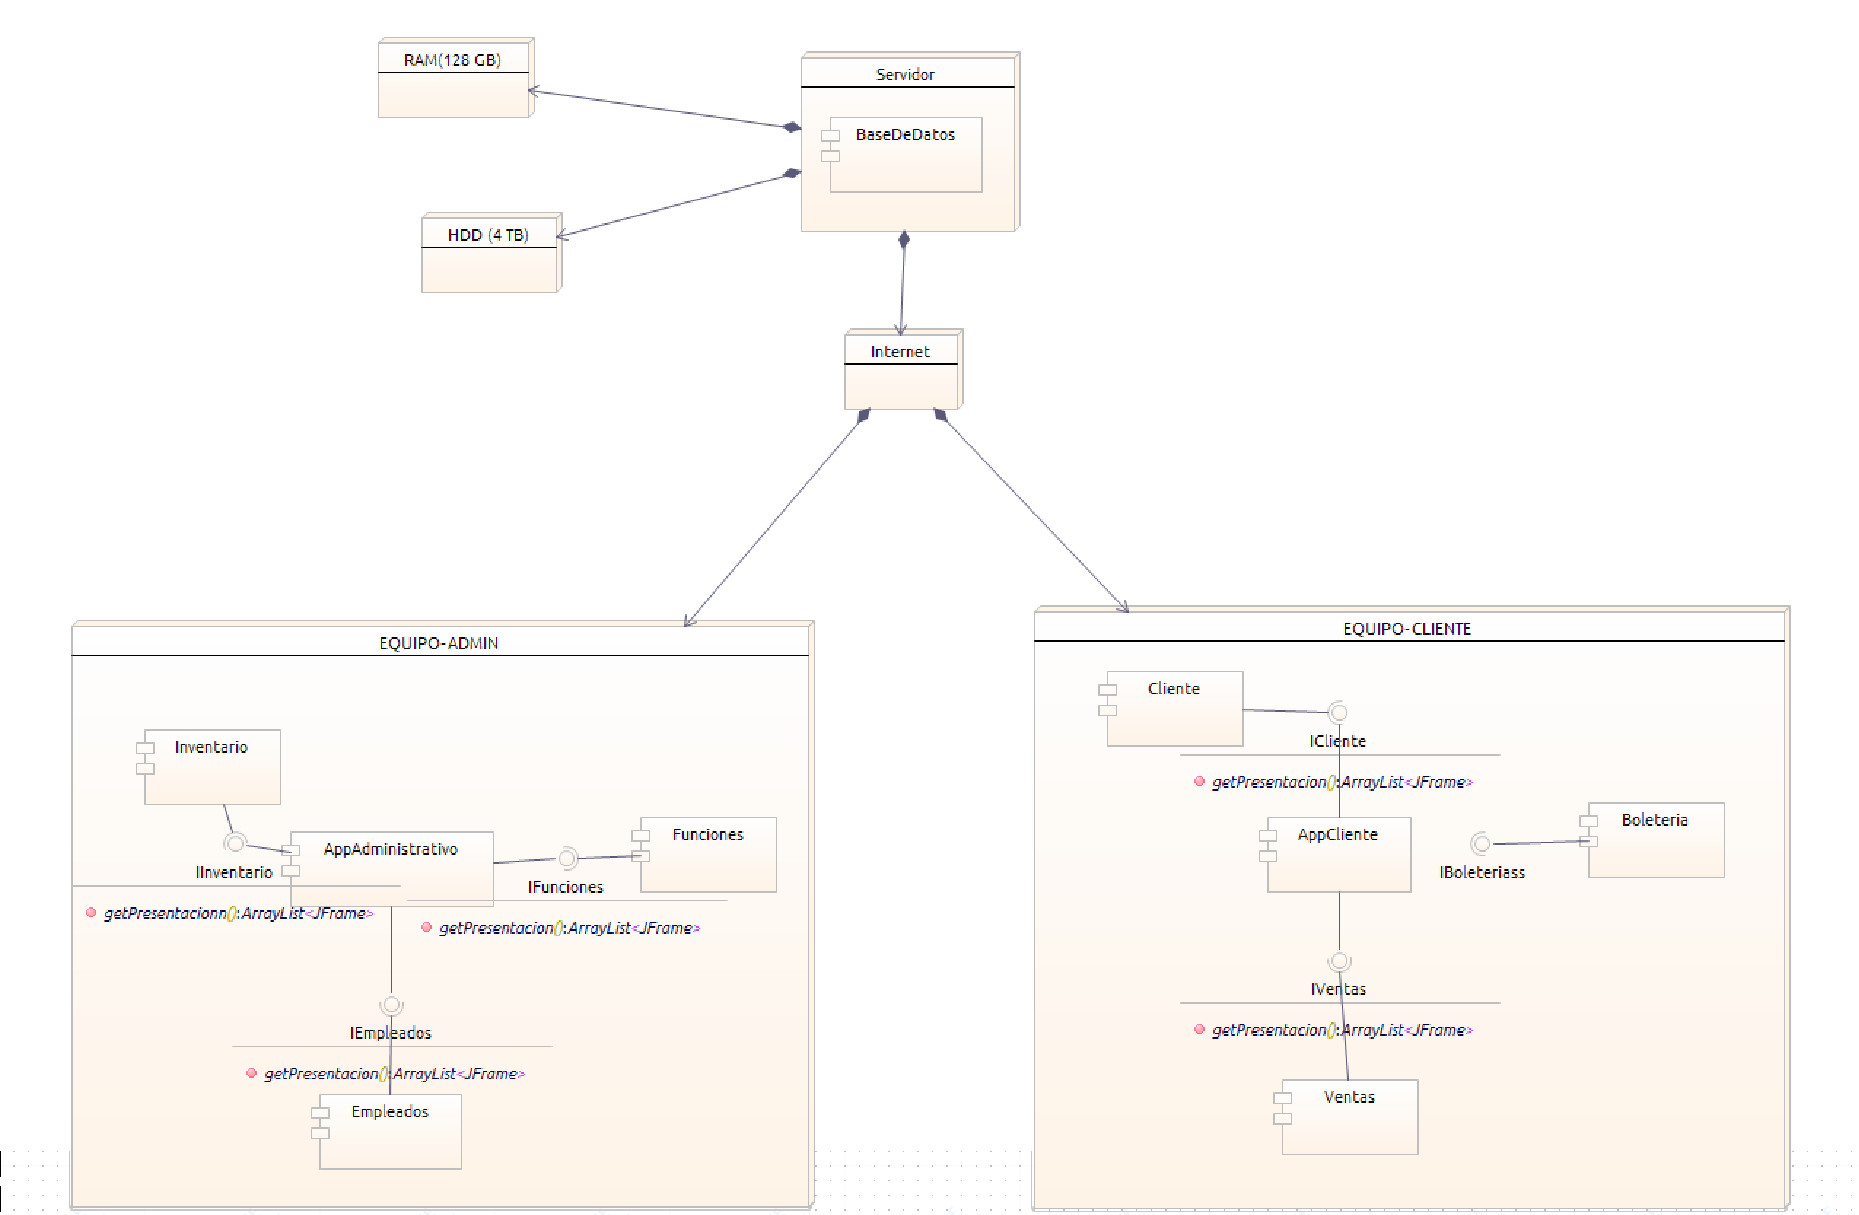
\includegraphics[scale=0.5]{diseno/nodos/img/diagramaNodos}
	\caption{Diagrama de Nodos}
\end{figure}
